\documentclass[12pt]{article}
\usepackage[superscript]{cite}   % remove to use brackets instead of superscripts in citations
\usepackage{graphicx}
\usepackage{fancyhdr}
\usepackage{xcolor}
\usepackage{indentfirst}
\usepackage[a4paper, portrait, margin=1in]{geometry}
\usepackage{lastpage}
\usepackage{float}
\usepackage{tabularx}
\pagestyle{fancy}
\fancyhf{}
\fancyhead[L]{Vupiter}
\fancyhead[R]{Project Proposal}
\rfoot{Page \thepage \hspace{1pt} of \pageref*{LastPage}}
\pagenumbering{arabic}
\newcolumntype{L}{>{\centering\arraybackslash}m{3cm}}
\usepackage[pdftex,bookmarks,pdfpagemode=UseOutlines,
    pdfauthor={Vupiter Team},
    pdftitle={Project Proposal},colorlinks=true, linkcolor=blue]{hyperref}
% removed colorlinks after bookmarks

\newcommand{\code}[1]{\texttt{\smaller #1}}

\setlength\parindent{5ex}
\setlength\parskip{2ex}
\newcommand\xrowht[2][0]{\addstackgap[.5\dimexpr#2\relax]{\vphantom{#1}}}
\newcommand{\fig}[1]{\centerline{\includegraphics{#1}}}

\DeclareGraphicsExtensions{.pdf, .jpg, .png}
%\setkeys{Gin}{width=0.85\textwidth}
\begin{document}
\begin{titlepage}
    \begin{center}
        \vspace*{1cm}
            
        \Huge
        \textbf{Vupiter DC Power Supply}
            
        \vspace{0.5cm}
        \large
        Date: \today
            
        \vspace{4.5cm}

        \textbf{Senior Design Project Proposal}
        
        \vspace{1cm}

        \textbf{Team Members:}\\
        Chase Flatau\\
        Alex Jones\\
        Rice Shelley\\
        Al Spies
        \vfill
            
            
        \vspace{0.8cm}
            
        
\includegraphics[width=0.4\textwidth]{university}
            
        \Large

        \textbf{Auburn University}\\
        Department of Electrical and Computer Engineering\\

            
    \end{center}
\end{titlepage}

\tableofcontents
\pagebreak

\section{Project Description}
DC power supplies are easily one of the most important pieces of test equipment 
in a lab while simultaneously being the most basic in concept. The focus of the 
Vupiter project will be to create a low-cost open-source versatile benchtop power 
supply. To make Vupiter versatile we will provide a computer interface that will 
allow power users to automate testing and data collection, in addition to the 
typical front-panel control. This computer interface will allow Vupiter to be 
useful in a much larger domain of experimentation than could be explored without a computer interface. 
Community expansion on this computer interface and the design as a whole will be 
enabled through thorough documentation at every stage. We will be documenting not 
just the technical details but also the decision making process along the way meaning 
Vupiter will be able to serve simultaneously as a useful lab tool and as a teaching 
tool. This level of documentation is the critical element frequently missing from most 
open source hardware projects, even other open source supplies, that prevents them 
from becoming truly community projects.
\section{Technical Description}
Vupiter will offer three independently isolated channels controllable both via a physical front panel and a USB connection. The supply will be powered by mains power, and each channel will deal with transforming that voltage separately. This choice means all three channels will have identical and parallel hardware, allowing for reuse in designs with more or less channels. Tying all three channels together will be one computer and user interface. With this in mind the design is broken down into three key sections: power supply design, microcontroller/software design, and user interface design.


\subsection{Constraints}
\subsubsection{Economical}
The primary purpose of a Vupiter power supply is to make desktop experimentation for 
hobbyists versatile, convenient, and low cost without greatly sacrificing performance. Devices 
with function and performance comparable to our targets are currently on the market for anywhere from \$300 to \$700. The aggressive initial constraint for this project is keeping build cost less than \$100 dollars to provide an affordable option for all electronic enthusiast, regardless of budgets. This difference in cost will be recouped by not having to make a profit, pay developers, or support users.

\subsubsection{Environmental}
Vupiter is intended for standard lab usage use so there’s an obvious ban on flagrantly toxic materials 
with all components. Toxic materials are an environmental concern not just due to user safety but also the possibility of these materials being discarded, and also the environmental effects of the components creation. Special attention will be paid in the component selection process so that we only consider safe and sustainable options where possible.

Energy efficiency is a major topic of concern globally. The design process will have to adhere to reasonable levels of efficiency. This will be accomplished by using switch-mode topologies for the majority of the voltage transformation. These will be followed by linear stages so that we can still meet the performance requirements.

\subsubsection{Manufacturability}
In order to ensure that both hobbyists and factories can produce the design, we will be constraining our PCBs to 2-layers with only one side populated by surface mount components. By avoiding through-hole components and only populating one side of the board we can drastically simplify automated PCB assembly. To assist hobbyists with the difficulty that surface mount components bring we will be limiting our passive component size to 0603 or above, and banning the use of ball grid arrays or other difficult to hand solder IC packages in favor of packages with exposed leads such as quad flat packs.

\subsubsection{Health and Safety}
Well-being of users, or anyone in close proximity, is the highest priority of the design process.Electrical constraints in this vein include fuses both in the first stage of each channel and the outputs, as well as opto-isolation of the front panel both from the channel outputs and mains voltage. Physical constraints in this vein limit sharp edges on the casement and require an ergonomic user interface to maximize comfort under standard usage.

\subsubsection{Usefulness}
From our team’s experience using power supplies we have identified a number of minimum performance targets that are necessary to keep Vupiter useful in a lab setting. This experience provides the already stated requirement of three independently isolated channels. Further constraints on these channels are that must be capable of 0-30V and 0-5A regulation at 10mV and 10mA resolution. Physically, the supply should sit flat on a level surface, and have a flat top, to allow for stacking of other instruments.

\subsection{Standards}
\subsubsection{UL 1310 Class 2 Power Units Standard for Safety}
The UL 1310 standard outlines and classifies power supplies. A class two power 
supply cannot exceed an output of 30 Volts and 8 Amperes. The Vupiter lab supply 
would be considered a class two power supply under the UL 1310 standard.
UL 1310 covers both indoor and outdoor power supplies however the primary environment
for the Vupiter lab supply is intended to be indoors. This class of power supply is 
intended primarily to provide power to low voltage electrical devices. 

\subsubsection{Universal Serial Bus Version 2.0}
The Vupiter power supply can be interfaced with a PC over the USB 2.0 protocol. Data 
transmission will be at a rate of 12 Mb/s. The Vupiter power supply will be a slave
device and have a USB type B port located on the front panel. This interface was selected over more traditional lab equipment interfaces such GPIB due to it's popularity in consumer hardware, and thus greater accessibility in the hobbyist market. Compliance with the standard is assured by the microcontroller vendor.

\subsubsection{USB Test and Measurement Class Specification}
USBTMC will be used on top of the USB 2.0 protocol for communication with the power supply. By supporting this interface we will gain access to plug and play communication, easing integration with various operating systems and languages. Compliance with this standard will be ensured by the senior design team. This requires the development of a driver set for our microcontroller choice and is enabled by the TMC standard being readily accessible on the internet.

\subsubsection{Standard Commands for Programmable Instruments (SCPI)}
SCPI will be used on top of USBTMC and it defines the individual commands for controlling programmable instruments. The Vupiter power supply will use SCPI as the top level command interface between itself and PC desktop software. The SCPI functionality class DCPSUPPLY will be implemented into the software. The DCPSUPPLY class will ensure that other SCPI DC power supply control software can be used with the Vupiter power supply. SCPI was selected over alternative standards such as VISA due to it's openness and human readability. Human readability and access to the standard simplifies the learning curve for custom script developers, a key component of hobbyist usage.

\subsection{Power Stages}
Benchtop power supplies are frequently attached to sensitive and poorly 
characterized devices meaning that the supply is subject to more rigorous 
and varied performance requirements than a typical specialized supply. 
These performance requirements can be roughly broken down into output noise 
and output step response requirements. These two criteria will be considered 
in addition to our budgetary and environmental requirements when evaluating 
designs. Four topologies for the power supply section of this project are 
explored and explained below, addressing these criteria. The final tallying 
of their pros and cons can be seen in \autoref{tab:power}.

\subsubsection{Topology 1 - Linear mode devices only}
This topology, seen in \autoref{fig:linear}, is by far the simplest as all it does is transform and rectify mains 
voltage, and then burn any excess voltage as heat in order to control the final 
output voltages. This results in a very high quality output, as there are no elements 
injecting switching noise and the entire voltage range is available for step response. 
Those benefits are exactly its downfall sadly, as the requirement on the transformer 
for it to work at 60 Hz requires that cycle by cycle it must be able to store a 
large amount of energy in it's magnetic field. This implies a physically large design, as 
the more energy that needs to be stored, the greater the amount of ferrous core that is needed. 
Not only does this make for bulky and heavy transformers, but it also greatly increases 
the cost. Aside from this, the linear element, shown in the diagram in red, also has issues. As we cannot adjust the output of the rectifier, that linear element has to 
turn all the excess voltage into heat. This means that the power supply running at 
a low voltage output but drawing high amperage would need to dissipate nearly 200 
Watts. This would undoubtedly require heat sinking and active cooling, further driving up 
the price and weight of this design.

\begin{figure}[H]
    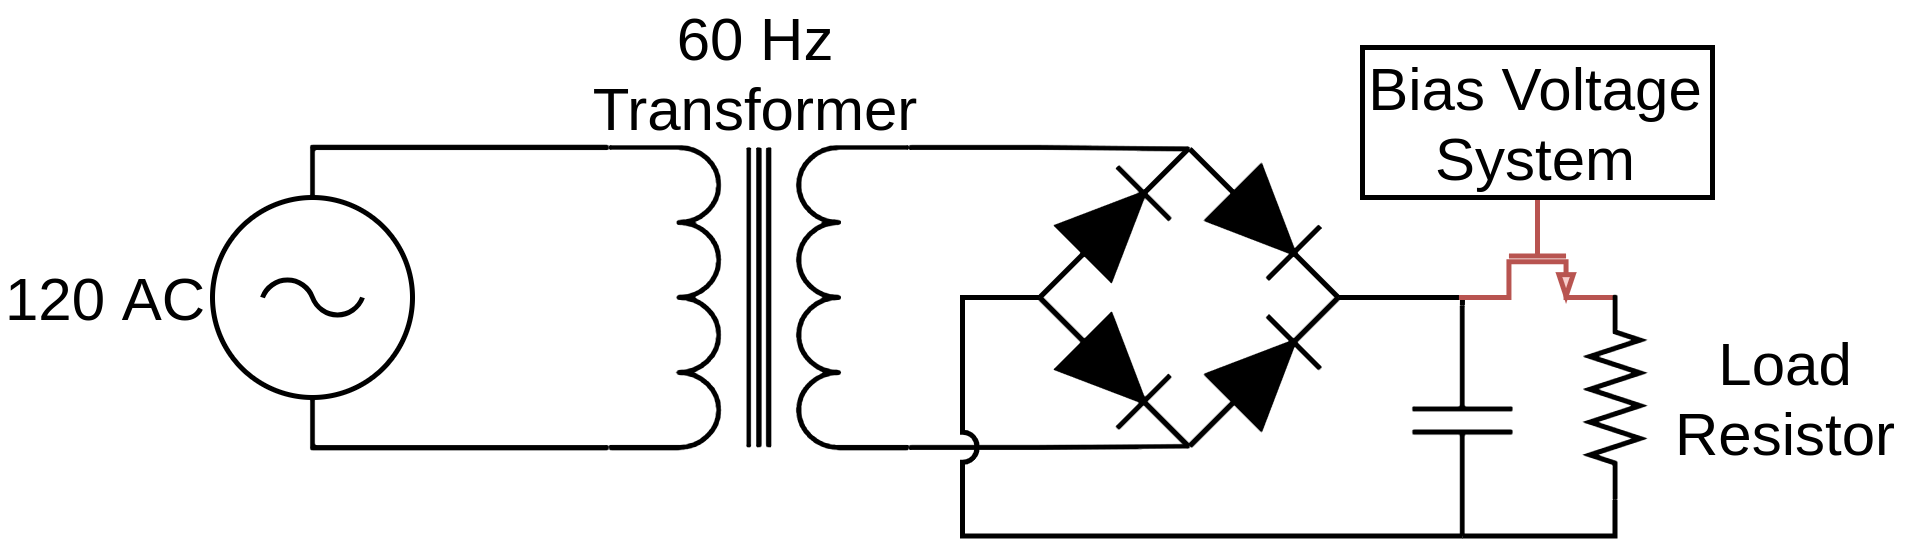
\includegraphics[width=\textwidth]{linear}
    \caption{Entirely linear mode design}
    \label{fig:linear}
\end{figure}

\subsubsection{Topology 2 - Switch mode devices only}
To address the issues with linear regulation, let's examine a purely switch mode 
regulator. As can be seen in \autoref{fig:switched}, line voltage is immediately rectified. 
This gives us an approximately 170 volt DC supply. From that 170 volt supply, we switch 
it at high frequency through a transformer. Due to this ability to increase the 
frequency the transformer operates at, we can decrease it's size and thus price.From 
the output we have to rectify again, and then we go on to our final regulation stage 
which is a buck converter. This buck converter is able to control the output voltage 
at high efficiency, but due to its requirement for high output capacitance, current 
limiting and voltage recovery speed suffer. Even worse, the buck converter both 
fails to filter noise from the first switched converter stage, and also injects 
noise at its switching frequency. This noise, and the poor current limiting results 
in a low quality output that would make this power supply useless or even dangerous to the device under test in a large number of applications. That being said, this design has extremely high efficiency, as no part of it is dissipating power intentionally. The high efficiency allows us to reduce the size(and thus cost) of some parts and completely eliminate other items such as heat sinks and fans.

\begin{figure}[H]
    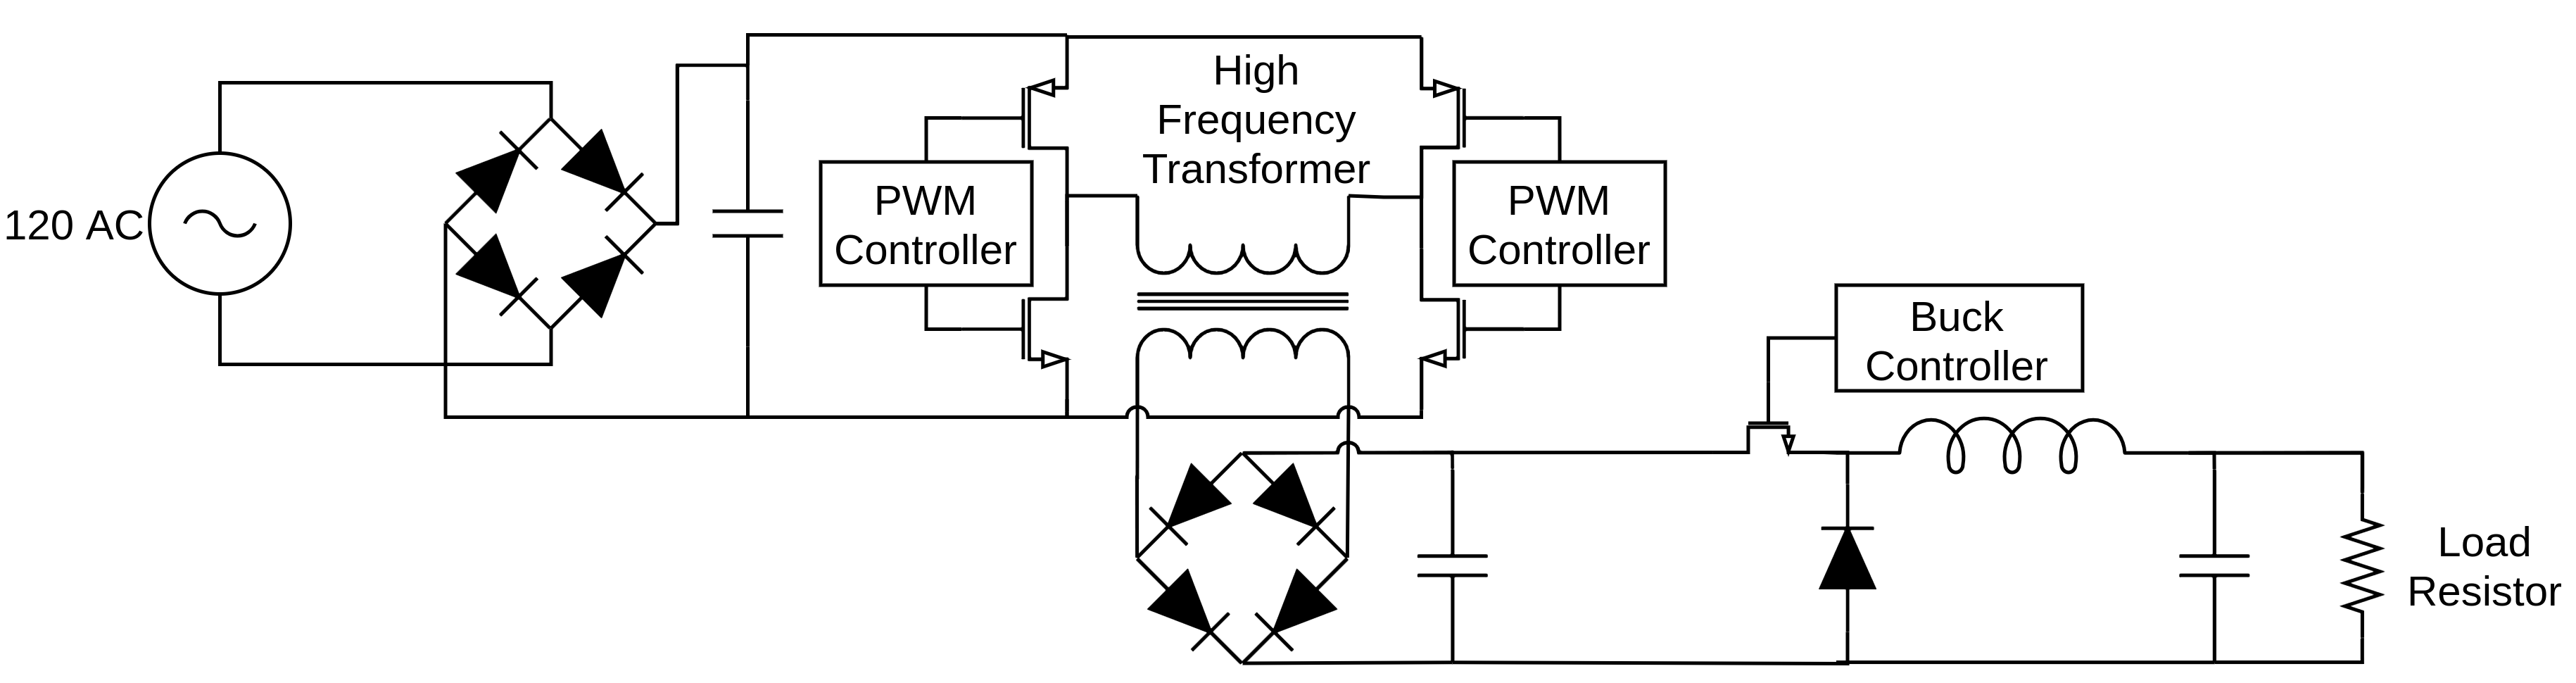
\includegraphics[width=\textwidth]{switched}
    \caption{Entirely switch mode design}
    \label{fig:switched}
\end{figure}
\subsubsection{Topologies 3 and 4 - Mixed mode supplies}

These two topologies are together as they share a single concept and block diagram, 
but there are major differences in their feedback loops and how they respond. 
As can be seen in \autoref{fig:mixed}, these topologies are composed of different pieces 
from topologies one and two, earning them their name as mixed mode rather than 
linear or switched exclusively. These two are using the high frequency transformer 
stage from the switch mode design, followed by a linear regulator on the output. 
This allows us to eliminate the high cost 60 Hz transformer while still maintaining 
the benefits of linear regulation. The switch mode elements here still inject noise, 
but as they are followed by a linear stage, that noise can be filtered both by passive 
elements and by the linear elements, ensuring a high quality output regulation.  

The first of our two topologies in this domain is a fixed mixed mode design. 
This means that the voltage output of the second rectifier is controlled to a 
fixed value, I.E. if the desired voltage is 20V, the transformer will target 25V 
and allow the additional 5V to be dissipated in the linear stage. The benefit 
here is higher efficiency than the linear only design as we can decrease the supply 
voltage at low output voltages while still maintaining strong regulation and step response.

The alternative to this is a floating mixed mode design whereby the output of the 
second rectifier is regulated to always be just slightly above the dropout of the 
linear stage. This ensures exceptionally high efficiency as the linear element is 
dissipating at most tens of watts even with a short circuit across its output. This  
becomes problematic when reacting to large step inputs both on the load or the command 
side, as the maximum positive output voltage slew is dictated by the switched elements 
rather than the linear elements. Another point off for this design is the difficulty of designing a floating switch mode section. This can drastically complicate feedback loops and if done improperly will result in an unstable output. Due to this, floating output voltages are infrequent, driving up 
the cost to design one as controller IC choice is limited.

\begin{figure}[H]
    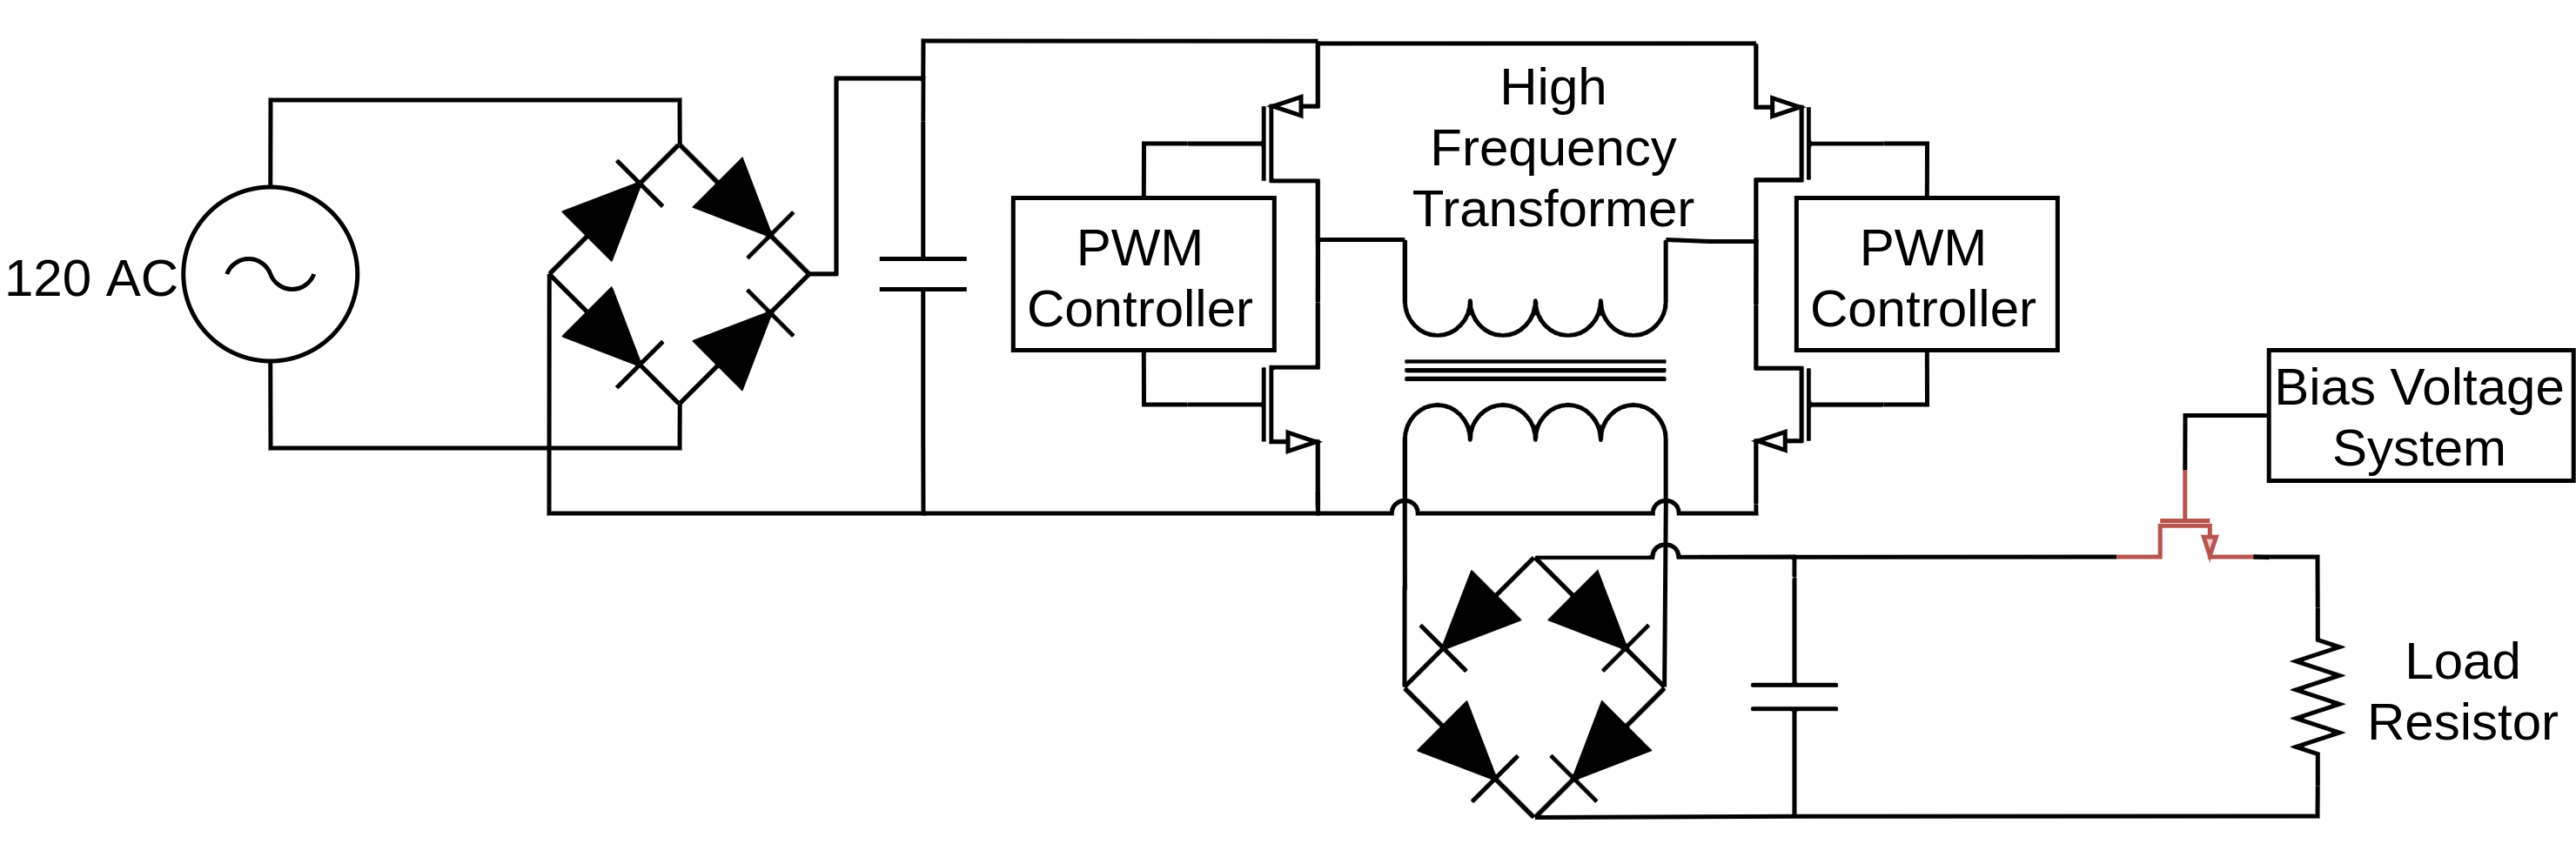
\includegraphics[width=\textwidth]{mixed}
    \caption{Mixed modality design}
    \label{fig:mixed}
\end{figure}
\begin{table}[H]
    \centering
\begin{tabular}{ |c|c||c|c|c|c|  }
    \cline{3-6}
    \multicolumn{1}{c}{}& \multicolumn{1}{c}{}&  \multicolumn{4}{|c|}{\textbf{Options}} \\
    \hline
    \textbf{Criteria} & \textbf{Weight} & Linear & SMPS & Fixed Mixed & Floating Mixed \\ 
    \hline
    Efficiency & 1 & {-}{-}{-} & 0 & {-}{-} & - \\
    Cost & 2 & {-}{-}{-} & 0 & {-} & {-}{-} \\
    Noise & 2 & ++ & 0 & + & + \\
    Step Response & 2 & ++ & 0 & ++ & + \\
    Design Effort & 1 & + & 0 & - & {-}{-} \\ 
    \hline
    \hline
    \multicolumn{2}{|c||}{+} & 9 & 0 & 6 & 4\\
    \multicolumn{2}{|c||}{0} & 0 & 5 & 0 & 0\\
    \multicolumn{2}{|c||}{-} & 9 & 0 & 4 & 7\\
    \hline
    \hline
    \multicolumn{2}{|c||}{\textbf{Net Score}} & 0 & 0 & 2 & -3\\
    \hline
\end{tabular}
\caption{Pugh table for power stage topology selection}
\label{tab:power}
\end{table}


\subsection {Micro-Controller}

Price and USB support were the biggest concerns when considering a MCU for the project. Four Candidates were considered, and the results are explained below with a summary in \autoref{tab:micro}.The Raspberry PI was not a strong candidate due to its price and lack of analog peripherals. The STM32’s tool chain lacks linux support and is not especially intuitive. ATmega 2560, despite its huge set of software libraries lacks USB support which will be important for the communication between power supply and the PC. The STM32 line of chips also has multiple viable candidates but the tool and library support is lacking. The ATmega Samd51 cuts down the middle with decent tools and all the required hardware at a good price point. In addition to the above mentioned benefits the Samd51 does not require as many external components, allowing us to simplify PCB design. A development board has been selected for the Samd so that software development may begin before the PCB is designed.

\begin{table}[H]
    \centering
    \begin{tabular}{ |c|c||c|c|c|c|  }
    \cline{3-6}
    \multicolumn{1}{c}{}& \multicolumn{1}{c}{}&  \multicolumn{4}{|c|}{\textbf{Options}} \\
    \hline
    \textbf{Criteria} & \textbf{Weight} & ATMega Samd51 & ATMega 2560 & Raspberry Pi & STM32 \\ 
    \hline
    ADC and DAC & 3 & + & 0 & - & + \\
    Price & 5 & + & 0 & - & + \\
    USB support & 5 & + & 0 & + & + \\
    Tools & 2 & 0 & 0 & + & + \\
    Libraries & 1 & - & 0 & + & - \\ 
    \hline
    \hline
    \multicolumn{2}{|c||}{+} & 13 & 0 & 8 & 13\\
    \multicolumn{2}{|c||}{0} & 1 & 5 & 0 & 0\\
    \multicolumn{2}{|c||}{-} & 1 & 0 & 8 & 3\\
    \hline \hline
    \multicolumn{2}{|c||}{\textbf{Net Score}} & 12 & 0 & 0 & 10\\
    \hline
\end{tabular}
\caption{Pugh table for micro-controller selection }
\label{tab:micro}
\end{table}

\subsection{User Interface}

The user interface can be broken into two subsections, the information display and the controls. The main criteria for these two subsections are cost, implementation difficulty, and usability. For the display, three options were considered: seven segment displays, a TFT screen, and a touchscreen. The touchscreen simplifies our component count by unifying the display and the interface, but it is both expensive and lacks the tactile feedback that is essential to good user interaction. Seven-segment displays are a classic and robust solution but the shear quantity for three channels would be too expensive and cluttered. The intermediary solution of a non-touch screen and a discrete interface fixes these issues and is relatively inexpensive. These results are summarized in \autoref{tab:display}.

\begin{table}[H]
    \centering
\begin{tabular}{ |c|c||L|L|L|  }
    \cline{3-5}
    \multicolumn{1}{c}{}& \multicolumn{1}{c}{}&  \multicolumn{3}{|c|}{\textbf{Options}} \\
    \hline
    \textbf{Criteria} & \textbf{Weight} & LTC-4627JR 4 Digit Seven Segment Display & Hx8357B TFT Screen & Mikroe-495 touchscreen display \\ 
    \hline
    Price & 3 & 0 & + & -  \\
    Usability & 2 & - & 0 & + \\
    Quality & 1 & - & 0 & + \\
    Durability & 1 & + & 0 & - \\
    Implementation & 2 & + & 0 & - \\ 
    \hline
    \hline
    \multicolumn{2}{|c||}{+} & 3 & 3 & 3\\
    \multicolumn{2}{|c||}{0} & 1 & 4 & 0\\
    \multicolumn{2}{|c||}{-} & 3 & 0 & -6\\
    \hline \hline
    \multicolumn{2}{|c||}{\textbf{Net Score}} & 0 & 3 & -3\\
    \hline
\end{tabular}
\caption{Pugh table for display selection }
\label{tab:display}
\end{table}

For the user interface, three options were considered against the same criteria, these being: encoder, matrix button array, and a touchscreen. The touchscreen has the same issues as above of being expensive and lacking tactile feedback. A keypad, while robust and relatively cheap, would make fine adjustments difficult and menu navigation unintuitive. This leaves us with encoders, which allow for fine adjustment, provide tactile feedback, and are relatively cheap. Intuitive menu navigation can 
be achieved by having three encoders, two dedicated to voltage and current control with the third managing the switching between channels and any other menu options. These results are summarized in \autoref{tab:control}.
\begin{table}[H]
    \centering
\begin{tabular}{ |c|c||L|L|L|  }
    \cline{3-5}
    \multicolumn{2}{c}{} &  \multicolumn{3}{|c|}{\textbf{Options}} \\
    \hline
    \textbf{Criteria} & \textbf{Weight} & 4x3 Matrix Keypad & Encoders & Mikroe-495 touchscreen display \\ 
    \hline
    Price & 3 & - & + & -  \\
    Usability & 2 & - & + & 0 \\
    Quality & 1 & - & + & - \\
    Durability & 1 & 0 & + & - \\
    Implementation & 2 & 0 & + & - \\ 
    \hline
    \hline
    \multicolumn{2}{|c||}{+} & 0 & 9 & 0\\
    \multicolumn{2}{|c||}{0} & 2 & 0 & 1\\
    \multicolumn{2}{|c||}{-} & -6 & 0 & -7\\
    \hline \hline
    \multicolumn{2}{|c||}{\textbf{Net Score}} & -6 & 9 & -7\\
    \hline
\end{tabular}
\caption{Pugh table for user interface selection }
\label{tab:control}
\end{table}

\section{Management Approach}

Our team holds weekly meetings on Wednesday morning at 9 AM to discuss progress and work on team tasks.These meeting are done on our discord server which is also how we communicate outside of meetings. Documentation and version control is done through GitHub. The team is roughly split into two groups with Alex Jones and Chase Flatau working on power stages while Rice Shelley and Al Spies work on firmware. Each team communicates within separate channels for internal communication, and any major decisions or issues are run by the entire team at the weekly meetings. The overall project lead is Alex Jones.

\noindent 
Meeting minutes are recorded weekly by Al Spies and can be accessed on our website: \url{https://ams0187.github.io/Vupiter/}

\noindent
All files, including this proposal are hosted on our github:\\
\url{https://github.com/ams0187/Vupiter}
\section{Budget}
In order to be competitive with market alternatives, our target cost is \$100. 
Each member will contribute \$25 to purchase the necessary materials. The finished product will
be assembled in each members’ private workspace; therefore, consumables such as solder will count as
donations but will still be counted into the final price. The current targets for each subsection
are: \$25 are for front panel display and button/knobs, \$50 for the power stages
and PCBs, and \$25 for the casing of the supply.

\section{Timeline}
The project timeline can be accessed here: \url{https://aub.ie/vupiterTL}
\section{Facilities}
The facilities that will be utilized are Auburn’s SPaRC Lab and individual members’ home workshops. In the event that these labs are insufficient, the ECE shop will be contacted for assistance
\section{Disposition Agreement}
All members agree that the final physical product will donated to SPaRC and that all documentation, code, and intellectual property will be released on GitHub under the MIT licence. By signing on the next page each member acknowledges and agrees to the above statements.
\newpage

\begin{table}[H]
\begin{tabular}{ l | c }
    \textbf{Name} & \textbf{Signature} \\
    & \\ [5ex]
    Chase Flatau &\\[10ex]
    Alex Jones &\\[10ex]
    Rice Shelley &\\[10ex]
    Al Spies &\\[10ex]

\end{tabular}
\end{table}
\end{document}